\documentclass[tikz,border=5pt]{standalone}
\usepackage{times}
\usetikzlibrary{arrows.meta,positioning,calc}
\begin{document}
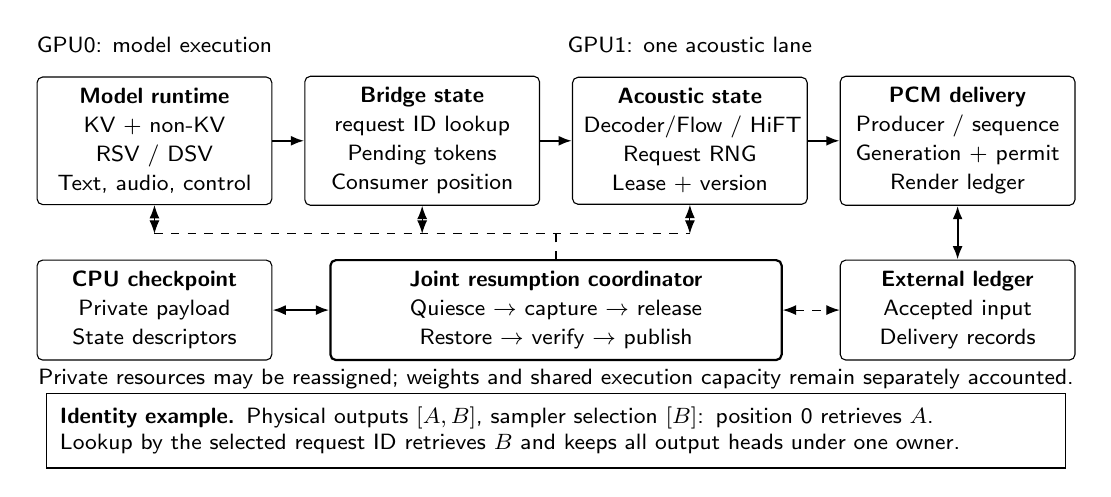
\begin{tikzpicture}[font=\sffamily\fontsize{8.5}{10.5}\selectfont,>={Latex[length=1.7mm]},
 stage/.style={draw,rounded corners=2pt,text width=2.7cm,minimum height=1.55cm,align=center,inner sep=4pt},
 lower/.style={draw,rounded corners=2pt,minimum height=1.2cm,align=center,inner sep=4pt}]
\node[stage] (m) at (1.45,0) {\textbf{Model runtime}\\KV + non-KV\\RSV / DSV\\Text, audio, control};
\node[stage] (b) at (4.85,0) {\textbf{Bridge state}\\request ID lookup\\Pending tokens\\Consumer position};
\node[stage] (a) at (8.25,0) {\textbf{Acoustic state}\\\mbox{Decoder/Flow / HiFT}\\Request RNG\\Lease + version};
\node[stage] (d) at (11.65,0) {\textbf{PCM delivery}\\\mbox{Producer / sequence}\\\mbox{Generation + permit}\\Render ledger};
\foreach \x/\y in {m/b,b/a,a/d}{\draw[->,thick] (\x.east)--(\y.west);}
\node[font=\sffamily\fontsize{8}{9}\selectfont,anchor=south] at (1.45,1.0) {GPU0: model execution};
\node[font=\sffamily\fontsize{8}{9}\selectfont,anchor=south] at (8.25,1.0) {GPU1: one acoustic lane};
\node[lower,text width=2.7cm] (cpu) at (1.45,-2.15) {\textbf{CPU checkpoint}\\Private payload\\State descriptors};
\node[lower,text width=5.45cm,line width=.8pt] (c) at (6.55,-2.15) {\textbf{Joint resumption coordinator}\\Quiesce $\rightarrow$ capture $\rightarrow$ release\\Restore $\rightarrow$ verify $\rightarrow$ publish};
\node[lower,text width=2.7cm] (l) at (11.65,-2.15) {\textbf{External ledger}\\Accepted input\\Delivery records};
\draw[<->,thick] (cpu.east)--(c.west);
\draw[dashed] (c.north)--(6.55,-1.18);
\draw[dashed] (1.45,-1.18)--(8.25,-1.18);
\foreach \n in {m,b,a}{\draw[<->,dashed] (\n.south)--(\n.south |- 0,-1.18);}
\draw[<->,thick] (d.south)--(l.north);
\draw[<->,dashed] (c.east)--(l.west);
\node[font=\sffamily\fontsize{7.8}{9}\selectfont,align=center] at (6.55,-3.02) {Private resources may be reassigned; weights and shared execution capacity remain separately accounted.};
\node[draw,text width=12.6cm,align=left,font=\sffamily\fontsize{8}{9.5}\selectfont,inner sep=5pt] at (6.55,-3.68) {\textbf{Identity example.} Physical outputs $[A,B]$, sampler selection $[B]$: position 0 retrieves $A$.\\Lookup by the selected request ID retrieves $B$ and keeps all output heads under one owner.};
\end{tikzpicture}
\end{document}
